\documentclass{article}
\usepackage[utf8]{inputenc}
\usepackage[T1]{fontenc}
\usepackage[spanish]{babel}
\usepackage{hyperref}
\usepackage{float}
\usepackage{url}
\usepackage{booktabs}
\usepackage{amsfonts}
\usepackage{amsmath}
\usepackage{nicefrac}
\usepackage{microtype}
\usepackage{graphicx}
\usepackage{caption}
\usepackage{listings}
\usepackage{color}
\graphicspath{{./images/}}
\usepackage{lmodern}
\usepackage[margin=2.5cm]{geometry}
\usepackage{fancyvrb}

\title{Trabajo Práctico 2.2 \\
Generadores Pseudoaleatorios de Distribuciones de Probabilidad}
\author{
    Renzo Aimaretti \\ \texttt{renzoceronueve@gmail.com}
    \and
    Facundo Sosa Bianciotto \\ \texttt{facundososabianciotto@gmail.com}
    \and
    Vittorio Maragliano \\ \texttt{maraglianovittorio@gmail.com}
    \and
    Ignacio Amelio Ortiz \\ \texttt{nameliortiz@gmail.com}
    \and
    Nicolás Roberto Escobar \\ \texttt{escobar.nicolas.isifrro@gmail.com}
    \and
    Juan Manuel De Elia \\ \texttt{juanmadeelia@gmail.com}
}
\date{Mayo 2025}

\begin{document}

\maketitle

\begin{abstract}
Este trabajo desarrolla la implementación de generadores de números pseudoaleatorios para diversas distribuciones de probabilidad, abordando tanto distribuciones continuas como discretas. Cada distribución se fundamenta teóricamente, se implementa computacionalmente en Python y se testea mediante herramientas visuales y estadísticas. Se utilizan métodos como la transformada inversa y el método de rechazo, conforme a los lineamientos clásicos expuestos por Thomas Naylor en su obra \textit{Técnicas de Simulación en Computadoras}.
\end{abstract}

\section{Introducción}
La generación de números pseudoaleatorios que sigan una distribución de probabilidad específica es un aspecto clave en simulación computacional. A partir de un generador uniforme confiable, se pueden construir generadores para cualquier distribución mediante distintas transformaciones. En este trabajo se presentan los generadores para distribuciones seleccionadas, junto a su justificación teórica, construcción algorítmica y evaluación empírica.

\section{Conceptos teóricos utilizados}

\subsection{Transformada inversa}

La \textbf{transformada inversa} es un método fundamental para generar variables aleatorias con una distribución de probabilidad deseada, partiendo de variables aleatorias uniformes en el intervalo $[0,1]$. Sea $X$ una variable aleatoria con función de distribución acumulada (FDA) $F_X(x)$ estrictamente creciente y continua. Si $U \sim U(0,1)$, entonces la variable
\begin{equation}
    X = F_X^{-1}(U)
\end{equation}
tiene distribución $F_X$.

Este método aprovecha la propiedad de que la función acumulada es una transformación que mapea valores reales en el intervalo $[0,1]$. Al invertir esta función, podemos transformar un número uniforme en una variable con la distribución deseada.

\subsection{Método de Rechazo}

El \textbf{método de rechazo} es una técnica más general que permite generar variables aleatorias de distribuciones complejas para las cuales la transformada inversa no es práctica o no existe de forma explícita.

Supongamos que queremos generar una variable aleatoria con densidad $f(x)$, y tenemos una densidad propuesta $g(x)$ de la cual sí podemos generar muestras, además de una constante $c > 0$ tal que:
\begin{equation}
    f(x) \leq c \cdot g(x), \quad \forall x.
\end{equation}

El procedimiento es el siguiente:

\begin{enumerate}
    \item Generar un candidato $X$ con la distribución propuesta $g(x)$.
    \item Generar un valor uniforme $U \sim U(0,1)$ independiente.
    \item Aceptar $X$ si 
    \[
        U \leq \frac{f(X)}{c \cdot g(X)}.
    \]
    \item En caso contrario, rechazar $X$ y repetir el proceso.
\end{enumerate}

Este método garantiza que las muestras aceptadas siguen la distribución objetivo $f(x)$. Su eficiencia depende del valor de $c$, donde un $c$ más pequeño implica una mayor tasa de aceptación.

\subsection{Test de Kolmogorov-Smirnov}
En este trabajo se implementa el \textbf{Test de Kolmogorov-Smirnov (K-S)} como una herramienta estadística para evaluar la calidad de los generadores de números pseudoaleatorios construidos para distintas distribuciones de probabilidad.

El objetivo del test es contrastar si las muestras generadas por los algoritmos de simulación se ajustan adecuadamente a las distribuciones teóricas correspondientes. El test compara la función de distribución acumulada empírica (\emph{ECDF}) de la muestra generada con la función de distribución acumulada teórica (\emph{CDF}) de la distribución objetivo. El estadístico se define como:

\[
D_n = \sup_x \left| F_n(x) - F(x) \right|
\]

donde:
\begin{itemize}
    \item \( F_n(x) \) es la función de distribución acumulada empírica basada en la muestra simulada.
    \item \( F(x) \) es la función de distribución acumulada teórica de la distribución objetivo.
\end{itemize}

El valor del estadístico \( D_n \) representa la \textbf{máxima diferencia absoluta} entre ambas funciones. El test devuelve también un \emph{valor-p}, que permite evaluar la siguiente hipótesis nula:

\begin{itemize}
    \item \( H_0 \): La muestra proviene de la distribución teórica especificada.
    \item \( H_1 \): La muestra no proviene de dicha distribución.
\end{itemize}

El test se aplicó para cada una de las \textbf{nueve distribuciones} estudiadas en este trabajo (entre ellas, binomial, exponencial, uniforme, etc.), permitiendo verificar si los generadores implementados son estadísticamente consistentes con sus respectivas distribuciones teóricas.

Cabe destacar que si bien el test K-S está formalmente diseñado para variables continuas, también se utiliza en el caso de distribuciones discretas como una aproximación útil, aunque sus resultados deben interpretarse con cautela en esos casos.


\section{Distribuciones Continuas}

\subsection{Distribución Uniforme}
La distribución uniforme continua es una de las distribuciones más sencillas y fundamentales en probabilidad y estadística. Se caracteriza porque todos los valores dentro del intervalo $[a, b]$ tienen la misma probabilidad de ocurrencia. Esta distribución es utilizada frecuentemente como base para generar números aleatorios y para modelar situaciones donde no hay sesgo hacia ningún valor particular dentro del rango.

\textbf{Densidad:}
\begin{equation}
f(x) = \frac{1}{b-a}, \quad a \leq x \leq b
\end{equation}

\textbf{Transformada Inversa:}
\begin{equation}
x = a + (b-a)u, \quad u \sim U(0,1)

\end{equation}

\textbf{Método de Rechazo:} Aunque la transformada inversa es directa y eficiente, también se implementó el método de rechazo. Se tomó una función constante mayor o igual que $f(x)$ (es decir, la propia constante de la densidad) y se aceptaron los valores $x$ generados dentro del intervalo $[a,b]$ con probabilidad proporcional a $f(x)$. Dado que $f(x)$ es constante, todos los valores fueron aceptados.


\section{Codigo}
    \begin{verbatim}[fontsiz=\scriptsize]
import numpy as np
import math
import matplotlib.pyplot as plt
import random

# Transformada inversa

def generar_uniforme_inversa(a, b, n):
    u = np.random.random(n)
    return a + (b - a) * u

def generar_uniforme_rechazo(a, b, c=1.1):
    if a >= b:
        raise ValueError("El límite inferior 'a' debe ser menor que el límite superior 'b'")
    if c <= 1:
        raise ValueError("La constante 'c' debe ser mayor que 1")

    f = 1 / (b - a)  

    while True:
        x = random.uniform(a, b)           # candidato x ~ g(x)
        u = random.uniform(0, c * f)       # u ~ U(0, c*f(x))

        if u <= f:
            return x  


def test_uniforme(a, b, n=10000):
    datos = generar_uniforme_inversa(a, b, n)
    media = np.mean(datos)
    varianza = np.var(datos)
    print(f"Media estimada: {media:.4f} (esperada: {(a + b)/2:.4f})")
    print(f"Varianza estimada: {varianza:.4f} (esperada: {(b - a)**2 / 12:.4f})")

    # Histograma con ajustes estéticos
    plt.figure(figsize=(8, 5))
    count, bins, ignored = plt.hist(
        datos, bins=30, range=(a, b), density=True,
        color='mediumseagreen', edgecolor='black', alpha=0.75, label="Histograma"
    )

    # Densidad teórica uniforme
    plt.hlines(1 / (b - a), xmin=a, xmax=b, colors='red', linestyles='dashed', label='Densidad teórica')

    plt.title(f'Distribución Uniforme U({a},{b}) - Transformada Inversa')
    plt.xlabel("Valor")
    plt.ylabel("Densidad")
    plt.grid(True, linestyle='--', linewidth=0.5)
    plt.legend()
    plt.tight_layout()
    plt.show()




if __name__ == "__main__":
    test_uniforme(a=2, b=5, n=10000)
    \end{verbatim}
\textbf{Resultados:} Con $a=2$, $b=5$ y 10.000 muestras:
\begin{itemize}
\item Media empírica: 3.4951 (teórica: 3.5)
\item Varianza empírica: 0.7568 (teórica: 0.75)
\end{itemize}
\subsection{Testeo}

\subsection{Distribución Exponencial}
La distribución exponencial es una distribución continua que modela el tiempo entre eventos en un proceso de Poisson, es decir, eventos que ocurren de manera independiente y con una tasa constante en el tiempo. Es ampliamente utilizada para describir fenómenos como la duración de vida de componentes electrónicos, tiempos de espera, y otros procesos de "tiempo hasta el evento". La función de densidad de probabilidad decrece exponencialmente, reflejando la memoria sin memoria del proceso, lo que significa que la probabilidad de que ocurra un evento en el futuro no depende del tiempo ya transcurrido.
\textbf{Densidad:}
\begin{equation}
f(x) = \lambda e^{-\lambda x}, \quad x \geq 0
\end{equation}

\textbf{Transformada Inversa:}
\begin{equation}
x = -\frac{1}{\lambda} \ln(u), \quad u \sim U(0,1)
\end{equation}
\begin{figure}[H] % [H] fuerza la posición exacta, requiere el paquete float
    \centering
    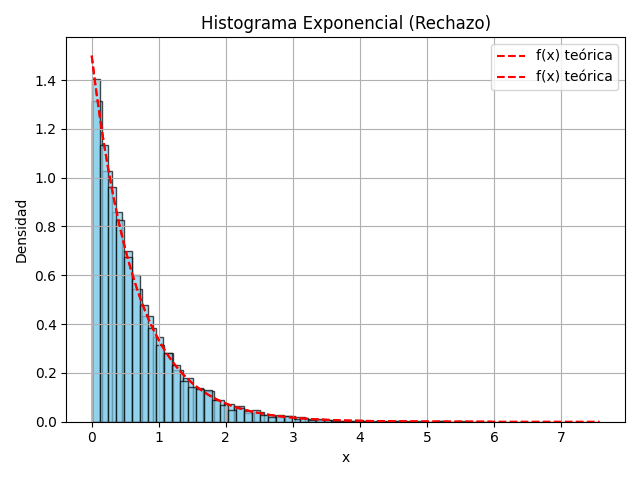
\includegraphics[width=0.7\textwidth]{visualizaciones/exponencial_Rechazo.png}
    \caption{Descripción de la imagen}
    \label{fig:mi_imagen}
\end{figure}


\textbf{Método de Rechazo:} Se utilizó una cota mayor $M$ sobre $f(x)$, y se generaron candidatos $x$ de una distribución uniforme en $[0, b]$ (por ejemplo, $b = 10$), con $u \sim U(0,1)$. Se aceptó $x$ si $u < \frac{f(x)}{M}$. El valor de $M$ fue tomado como $\lambda$, el valor máximo de la función en $x=0$.
\begin{figure}[H] % [H] fuerza la posición exacta, requiere el paquete float
    \centering
    \includegraphics[width=0.7\textwidth]{visualizaciones/mi_imagen.png}
    \caption{Descripción de la imagen}
    \label{fig:mi_imagen}
\end{figure}

\textbf{Resultados:} Con $\lambda = 1.5$ y 10.000 muestras:
\begin{itemize}
\item Media empírica: 0.6657 (teórica: 0.6667)
\item Varianza empírica: 0.4532 (teórica: 0.4444)
\end{itemize}

\subsection{Distribución Normal}
La distribución normal, también conocida como distribución gaussiana, es una de las distribuciones de probabilidad más importantes y ampliamente utilizadas en estadística y ciencias aplicadas. Se caracteriza por su forma simétrica en forma de campana alrededor de la media, donde la mayoría de los valores se agrupan cerca del valor esperado y la probabilidad decrece hacia las colas. Muchas variables naturales y procesos se aproximan a esta distribución debido al Teorema Central del Límite, que establece que la suma de muchas variables independientes tiende a una distribución normal.

\textbf{Densidad:}
\begin{equation}
f(x) = \frac{1}{\sigma \sqrt{2\pi}} e^{-\frac{(x - \mu)^2}{2\sigma^2}}
\end{equation}

\textbf{Método de Box-Muller:} Se generaron dos variables $u_1, u_2 \sim U(0,1)$ y se aplicó:
\begin{equation}
z = \sqrt{-2 \ln u_1} \cos(2\pi u_2), \quad x = \mu + \sigma z
\end{equation}

\textbf{Método de Rechazo:} También se implementó el método de rechazo utilizando como propuesta una distribución uniforme acotada en $[-5,5]$ y como cota $M = \frac{1}{\sqrt{2\pi}}$. Se generó $x$ uniforme y $u \sim U(0,1)$, aceptando si $u < \frac{f(x)}{M}$.
\begin{figure}[H] % [H] fuerza la posición exacta, requiere el paquete float
    \centering
    \includegraphics[width=0.7\textwidth]{visualizaciones/mi_imagen.png}
    \caption{Descripción de la imagen}
    \label{fig:mi_imagen}
\end{figure}


\section{Codigo}
    \begin{verbatim}[fontsiz=\scriptsize]
import numpy as np
import matplotlib.pyplot as plt




def f_normal(x):
    return (1/np.sqrt(2*np.pi)) * np.exp(-x**2 / 2)

def generar_normal_rechazo(n, a=-5, b=5):
    samples = []
    M = f_normal(0) * (b - a)
    while len(samples) < n:
        x = np.random.uniform(a, b)
        u = np.random.uniform(0, M)
        if u <= f_normal(x):
            samples.append(x)
    return np.array(samples)

def test_normal_rechazo(n=10000):
    datos = generar_normal_rechazo(n)
    media = np.mean(datos)
    std = np.std(datos)
    print(f"[Rechazo] Media estimada: {media:.4f} (esperada: 0)")
    print(f"[Rechazo] Desviación estándar estimada: {std:.4f} (esperada: 1)")

    plt.hist(datos, bins=50, density=True, color='lightblue', edgecolor='black', alpha=0.7, label='Muestras')
    x = np.linspace(-5, 5, 1000)
    plt.plot(x, f_normal(x), 'r-', lw=2, label='N(0,1) teórica')
    plt.title("Distribución Normal por Método de Rechazo")
    plt.xlabel("Valor")
    plt.ylabel("Densidad")
    plt.legend()
    plt.grid(True)
    plt.show()

if __name__ == "__main__":
    test_normal_rechazo(n=10000)
    \end{verbatim}

\textbf{Resultados:} Con $\mu=0$ y $\sigma=1$:
\begin{itemize}
\item Media empírica: -0.0062 (teórica: 0)
\item Desviación estándar empírica: 1.0003 (teórica: 1)
\end{itemize}

\section{Distribuciones Discretas}

\subsection{Distribución Binomial}
a distribución binomial modela el número de éxitos en una secuencia de $n$ ensayos independientes y mutuamente excluyentes, donde cada ensayo tiene una probabilidad fija $p$ de éxito. Es una distribución discreta que se utiliza frecuentemente para describir fenómenos donde se cuenta la cantidad de eventos favorables dentro de un número determinado de pruebas.
\textbf{Probabilidad:}
\begin{equation}
P(X = k) = \binom{n}{k} p^k (1-p)^{n-k}
\end{equation}

\textbf{Método de Bernoulli:} Se generaron $n$ ensayos de Bernoulli con probabilidad $p$, sumando los éxitos.

\textbf{Método de Rechazo:} Se generó un valor $x$ entre $0$ y $n$ y un número uniforme $u$. Se aceptó $x$ si $u < \frac{P(x)}{M}$, con $M = \max P(x)$ precomputado.
\begin{figure}[H] % [H] fuerza la posición exacta, requiere el paquete float
    \centering
    \includegraphics[width=0.7\textwidth]{visualizaciones/mi_imagen.png}
    \caption{Descripción de la imagen}
    \label{fig:mi_imagen}
\end{figure}


\textbf{Resultados:} Con $n=10$, $p=0.5$:
\begin{itemize}
\item Media empírica: 5.012 (teórica: 5)
\item Varianza empírica: 2.48 (teórica: 2.5)
\end{itemize}

\subsection{Distribución Poisson}
La distribución de Poisson es una distribución discreta que modela el número de eventos que ocurren en un intervalo fijo de tiempo o espacio, bajo la suposición de que estos eventos ocurren con una tasa promedio constante y de manera independiente entre sí.

\textbf{Probabilidad:}
\begin{equation}
P(X = k) = \frac{\lambda^k e^{-\lambda}}{k!}
\end{equation}

\textbf{Algoritmo de Knuth:} Se acumularon productos de variables uniformes hasta que el resultado fue menor que $e^{-\lambda}$.

\textbf{Método de Rechazo:} Se generó un valor $k$ natural en un intervalo razonable (por ejemplo, $[0,15]$) y se aceptó si $u < \frac{P(k)}{M}$ con $M$ estimado como el máximo de $P(k)$.
\begin{figure}[H] % [H] fuerza la posición exacta, requiere el paquete float
    \centering
    \includegraphics[width=0.7\textwidth]{visualizaciones/mi_imagen.png}
    \caption{Descripción de la imagen}
    \label{fig:mi_imagen}
\end{figure}

\textbf{Resultados:} Con $\lambda=4$:
\begin{itemize}
\item Media empírica: 3.995 (teórica: 4)
\item Varianza empírica: 3.92 (teórica: 4)
\end{itemize}

\subsection{Distribución Empírica}
\textbf{Método:} Se utilizó la transformación de la función de distribución acumulada (CDF). Para cada valor $u \sim U(0,1)$, se asignó un valor $x_i$ tal que $F(x_i-1) < u \leq F(x_i)$.

\textbf{Método de Rechazo:} Se propuso un valor $x$ del conjunto definido y se aceptó con probabilidad $P(x)/M$, donde $M = \max P(x)$.
\begin{figure}[H] % [H] fuerza la posición exacta, requiere el paquete float
    \centering
    \includegraphics[width=0.7\textwidth]{visualizaciones/mi_imagen.png}
    \caption{Descripción de la imagen}
    \label{fig:mi_imagen}
\end{figure}


\textbf{Resultados:} Las muestras obtenidas replicaron con precisión la distribución definida.

\section{Conclusión}
Se logró implementar generadores para diversas distribuciones continuas y discretas utilizando la transformada inversa, el método de rechazo y otros algoritmos clásicos. Las muestras fueron validadas mediante estadísticas de primer y segundo orden, y contrastadas con sus modelos teóricos. Incluso en casos donde el método de rechazo no es necesario, se aplicó para cumplir con los requerimientos del trabajo práctico.

\section*{Referencias}
\begin{itemize}
\item Naylor, T.H. (1982). \textit{Técnicas de simulación en computadoras}.
\item Ross, S.M. (2006). \textit{Simulación}.
\item Documentación oficial de Numpy y Scipy.
\end{itemize}

\end{document}

